\subsection{UC9 - Salvataggio della sessione}
\begin{figure}[h]
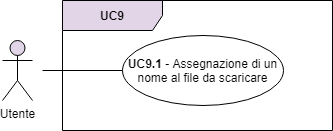
\includegraphics[width=10cm]{Section/Images/UC9.png}
\centering
\caption{UC9 - Salvataggio della sessione}
\end{figure}
\begin{itemize}
	\item \textbf{Attore primario}: Utente;
	\item \textbf{Precondizioni}: L'utente ha effettuato una sessione di lavoro, ossia:
	\begin{itemize}
	\item Caricato dei dati nel sistema ed eventualmente effettuato delle riduzioni dimensionali sui dati;
	\item Selezionato le visualizzazioni offerte dal sistema ed eventualmente modificato alcuni parametri di personalizzazione.
\end{itemize}	 
	\item \textbf{Postcondizioni}: L'utente possiede un file \glo{JSON} per il ripristino della sessione di lavoro;
	\item \textbf{Scenario principale}:
		\begin{enumerate}
			\item L'utente ha una sessione di lavoro aperta;
			\item L'utente seleziona la funzionalità "salva sessione";
			\item L'utente assegna un nome al file da scaricare [UC9.1];
			\item L'utente seleziona la directory in cui salvare il file.
		\end{enumerate}
\end{itemize}



\subsubsection{UC9.1 - Assegnazione di un nome al file da scaricare}

\begin{itemize}
	\item \textbf{Attore primario}: Utente;
	\item \textbf{Precondizioni}: L'utente ha una sessione di lavoro in corso; 
	\item \textbf{Postcondizioni}: L'utente modifica il nome d'assegnare al file da scaricare;
	\item \textbf{Scenario principale}: L'utente, attraverso l'apposito campo d'input, inserisce un nome a piacere d'assegnare al file da scaricare. Se non modificato, verrà mantenuto il nome assegnato di default.
\end{itemize}